\documentclass{article}
\usepackage[utf8]{inputenc}
\usepackage{amsmath,amsthm,amssymb,graphicx,mathtools,tikz,hyperref,enumerate, float}

\title{CAI Classification Problem\\Report 3: Implementation II}
\author{Nil Crespo-Peiró, Paco Rahn, Amin Ranem}
\date{26. January 2021}

\begin{document}

\maketitle

\section{Introduction}
Once the downsampled dataset has been loaded and the boilerplate code has been set up, the source code needed to be completed to be able to train different models in the future. Further, a first prototype for the Graphical User Interface (GUI) has been designed.
\noindent
In the following sections, the implementation details regarding the changed boilercode will be described and the structure of the user interface will be discussed.\\

\section{Implementation 2}
In this section, the final changes to the boilercode will be described.
\noindent
The second part of the report deals with the first prototype of the Graphical User Interface that has been divided into four main windows that will be explained in the corresponding section. 

\subsection{Final Code Structure}
One of the main issues using the whole Cholec80 dataset was the size of each video. Although they have been downsampled to 1 fps, each frame still needed to be resized to 224x224 pixels, in order to be used for transfer learning with PyTorch. With this approach, the Cholec80 dataset that will be used for training has been downsampled to 1 fps and each frame resized to 224x224 pixels. However, the whole transformed dataset is still too big to train with, given the time restriction of this project. Based on this problematic, from each video 2000 slices were randomly selected, if the video has more than 2000 frames, otherwise the whole video will be used for training. This has been realised using the \texttt{random} library from Python. The labels have been selected correspondingly. With these adjustments, the code base has been finished successfully and different models can be trained. In the next step, the first GUI prototype will be described, which will be connected to the source code in the next (future) steps.

\subsection{User Interface}
Since the GUI is an important thing to create that serves as a "bridge" between the source code and the users that will benefit from our work, a first design has been implemented using the \texttt{PySimpleGUI} library for Python.\\
\noindent
In order to make the life easier for the users of our Surgical Tool Recognition System, the GUI has to be designed in a way that it is firstly, appealing to the user, secondly, easy to understand/use and finally to ensure that the users give the inputs in the desired format in order to be able to make predictions with the trained model.
\noindent
In the next sections, a first prototype of the GUI will be presented, because it represents the foundation of the source code to be used in real case scenarios.

\subsubsection{First Window: Browse window}
In Figure \ref{fig:browse} one can clearly see an introduction message, followed by a brief description on how to proceed:
Either by writing a path to the video for which the user wants the surgical tools to be predicted or by browsing through his/her computer. \\
\noindent
Once this decision has been made the user can continue by hitting \texttt{Submit} or to \texttt{Cancel} and choose another video file.

\begin{figure}[H]
    \centering
    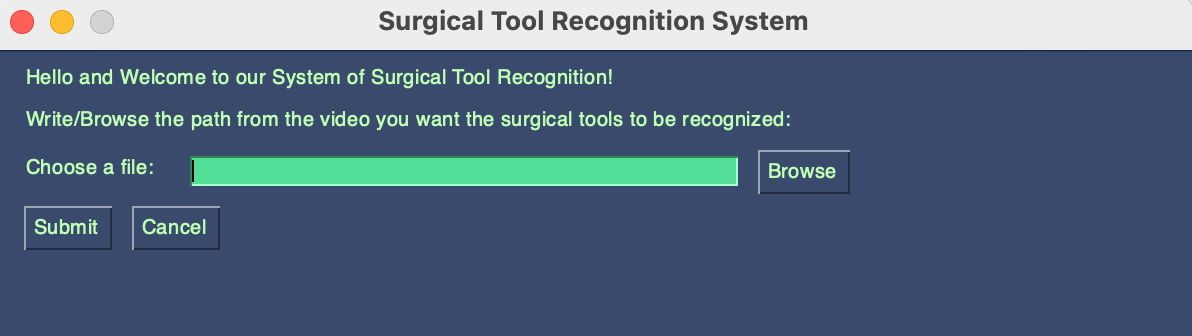
\includegraphics[width = \linewidth]{Browse_window.png}
    \caption{Browse window allowing users to select a video file to be tested}
    \label{fig:browse}
\end{figure}
\noindent
Once the user has pressed \texttt{Submit}, a "pop-up" appears in order to make sure this is the intended path to the video that should be further analysed. 

\begin{figure}[H]
    \centering
    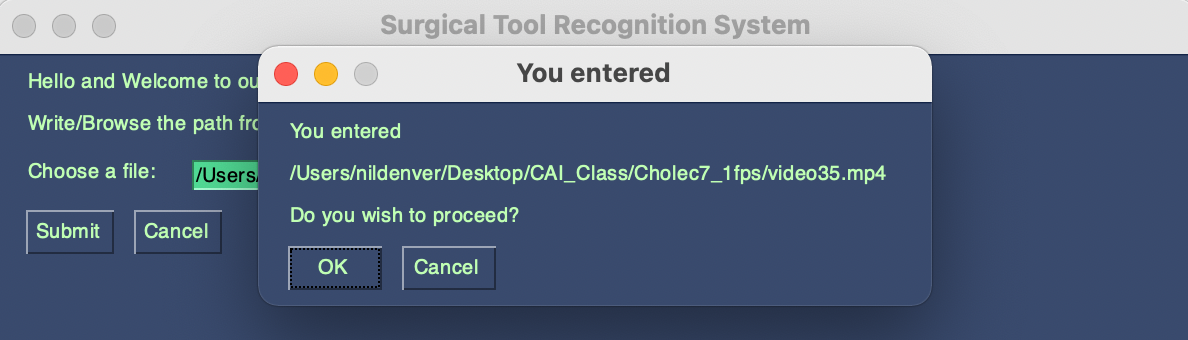
\includegraphics[width = \linewidth]{Confirm_window.png}
    \caption{Pop up window that ensures that the choice of the user is correct}
    \label{fig:confirm}
\end{figure}
\noindent
As one can see in Figure \ref{fig:confirm}, the popup shows the path that has been chosen along with a message reassuring that the decision was correct.

\subsubsection{Second Window - Model Flags, Losses and Specifications}
Once the user has pressed \texttt{OK} in the last popup window, the following loading window appears:

\begin{figure}[H]
    \centering
    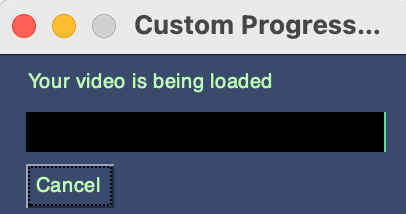
\includegraphics[width = 0.4\linewidth]{Loading_window.png}
    \caption{Loading window before choosing the parameters of the model}
    \label{fig:loading}
\end{figure}
\noindent
Once the loading bar has been filled, a Menu where the user can specify all the flags, parameters and options that could be chosen for the training of the model appears. 
Even though this window is already implemented, it will be redesigned and used to show the user the parameters of the pre-trained model which will be used for the actual prediction.

\begin{figure}[H]
    \centering
    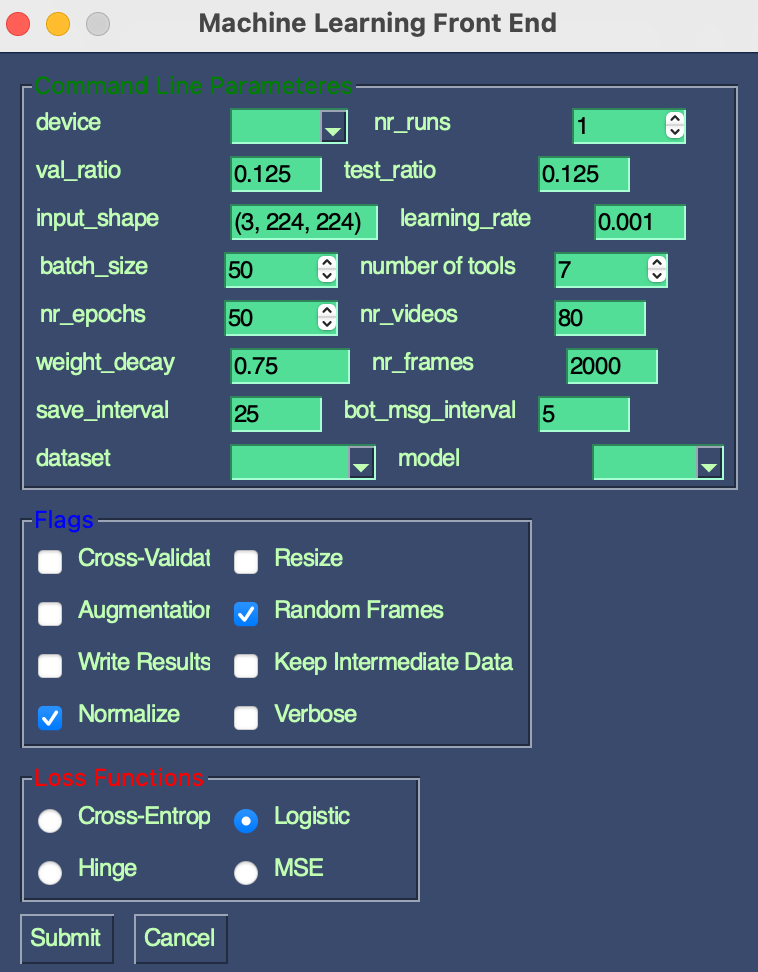
\includegraphics[width = 0.5\linewidth]{Parameter_window.png}
    \caption{Parameter window where all the flags and configurations can be chosen}
    \label{fig:parameter}
\end{figure}
\noindent
However, as we have already mentioned this will be redesigned, since the GUI will only be used for making predictions with a pre-trained model.

\subsubsection{Third Window - Output window}
In this third window, the user will face a similar window like the first one, but in this case he/she will have to write/browse to a folder where he/she wants the results of the Surgical Tool Recognition System to be saved. The window looks like the following:

\begin{figure}[H]
    \centering
    
\includegraphics[width = \linewidth]{Output_window.png}
    \caption{Output window where a folder where the results will be stored has to be decided}
    \label{fig:output}
\end{figure}
\noindent
As well as in the first window, a "pop-up" will appear to ensure the right location for storing the predictions.

\begin{figure}[H]
    \centering
    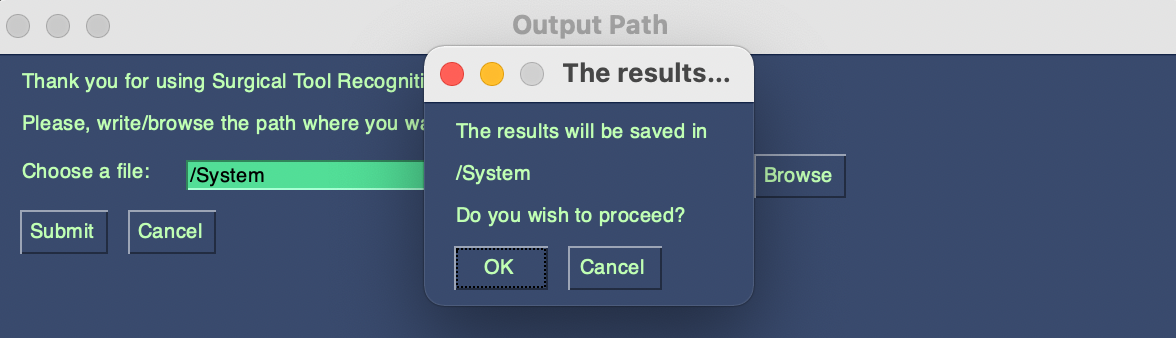
\includegraphics[width = \linewidth]{confirm_window2.png}
    \caption{Confirmation window in order to make sure that is the folder where the results have to be stored}
    \label{fig:confirm2}
\end{figure}
\noindent
Once again, the user will have a choice between the buttons \texttt{OK}, in case he/she wants to proceed, or \texttt{Cancel}, if the target folder is not the desired one.

\subsubsection{Fourth Window - Results window}
Right after the user has decided to proceed with that target path, another loading window will appear to indicate the computation of the predictions.

\begin{figure}[H]
    \centering
    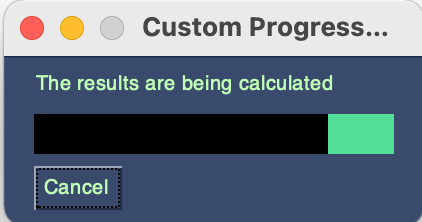
\includegraphics[width = 0.5\linewidth]{Loading_window2.png}
    \caption{Loading window before seeing the results}
    \label{fig:loading2}
\end{figure}
\noindent
Once the computation is finished, the final window will appear, showing the results. This window will show the results of the Surgical Tool Recognition System applied to the specified video. 

\begin{figure}[H]
    \centering
    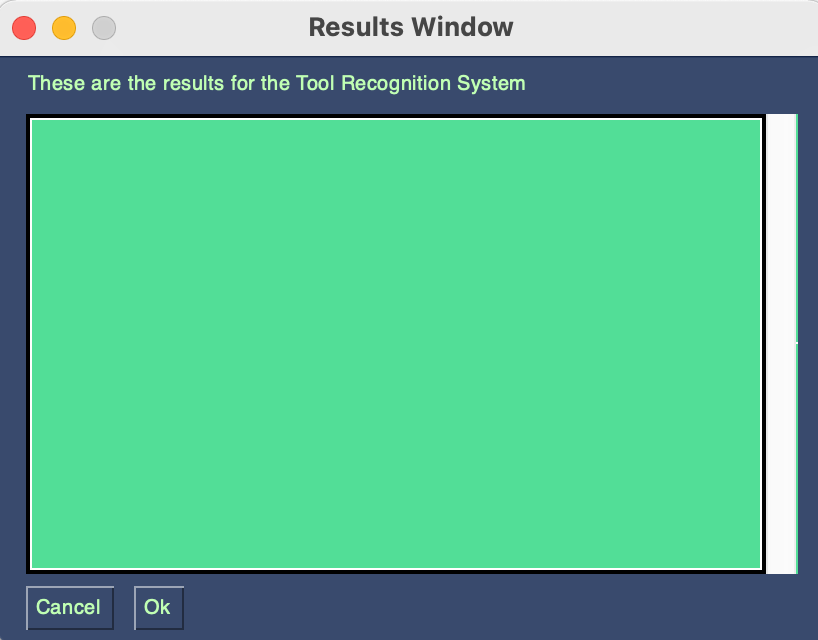
\includegraphics[width = 0.8\linewidth]{Results_window.png}
    \caption{Results window of our system}
    \label{fig:results}
\end{figure}
\noindent
In the text field, the results will be printed and the user will be able to analyse them aside from having them stored in the path they provided earlier.
\noindent
As we have already mentioned, this GUI is our first design and will be certainly modified/extended to improve it to the user and the source code's needs. The GUI needs still to be connected to the implemented source code.
\end{document}